\documentclass[preprint]{elsarticle}

%% Packages
\usepackage{listings}
\usepackage[cmex10]{amsmath}
\usepackage{url}
\usepackage{caption}
\usepackage{fancyvrb}
\usepackage{upquote}
\usepackage{multicol}
\usepackage{tikz}
\usepackage{scalerel}
\usepackage{longtable}
\usepackage{etoolbox}
\usepackage{float}
\usepackage{amssymb}
\usepackage{mathtools}
\usepackage{subcaption}
\usepackage{booktabs}
\usepackage{multirow}
\usepackage{algpseudocode}
\usepackage{calc,multicol}
\usepackage{algorithm}
\usepackage{setspace}
\usepackage{lastpage}
\usepackage{fancyhdr}
\usepackage{tikz}
\usepackage{pgfplots}
\pgfplotsset{compat=1.9}
\usetikzlibrary{patterns}

% \patchcmd{\thebibliography}{\clubpenalty4000}{\clubpenalty10000}{}{}
% \patchcmd{\thebibliography}{\widowpenalty4000}{\clubpenalty10000}{}{}
\usepackage{nasutil}

% start of the document
\begin{document}

% the title, author, abstract
\begin{frontmatter}
\title{Power-aware Allocation of Fault-tolerant Multirate AUTOSAR Applications}
\author{
\IEEEauthorblockN{
Nesredin Mahmud\IEEEauthorrefmark{1}, 
Guillermo Rodriguez-Navas\IEEEauthorrefmark{1},
Hamid Faragardi\IEEEauthorrefmark{2},
Saad Mubeen\IEEEauthorrefmark{1},
Cristina Seceleanu\IEEEauthorrefmark{1}}

\IEEEauthorblockA{\IEEEauthorrefmark{1}M{\"a}lardalen University, V\"aster{\aa}s, Sweden}
\IEEEauthorblockA{\IEEEauthorrefmark{2}KTH Royal Institute of Technology, Stockholm, Sweden}
\IEEEauthorblockA{ \IEEEauthorrefmark{1}\{firstname.lastname\}@mdh.se, \IEEEauthorrefmark{2}hrfa@kth.se}
} 

%mailto:faragardi@dps.uibk.ac.at
%KTH Royal Institute of Technology
%mahmud, guillermo.rodriguez-navas, hamid.faragardi, saad.mubeen, cristina.seceleanu
%\IEEEauthorrefmark{1}
% \author{
% \IEEEauthorblockN{Nesredin Mahmud\IEEEauthorrefmark{1}, Cristina Seceleanu\IEEEauthorrefmark{1}, Oscar Ljungkrantz\IEEEauthorrefmark{2}}
% \IEEEauthorblockA{\IEEEauthorrefmark{1}M\"{a}lardalen University, Sweden, \{nesredin.mahmud, cristina.seceleanu\}@mdh.se}
% \IEEEauthorblockA{\IEEEauthorrefmark{2}Volvo Group Trucks Technology, Sweden, oscar.ljungkrantz@volvo.com}
% %\IEEEauthorblockA{\IEEEauthorrefmark{2}Volvo Group Trucks Technology, Sweden, oscar.ljungkrantz@volvo.com}
% } 
\begin{abstract}
The growing complexity of automotive functionality has attracted revolutionary computing architectures such as mixed-criticality design, which enables effective consolidation of software applications with different criticality on shared execution platforms. The allocation of mixed-critical software application on the execution platform plays an important role in the design of predictable and resource-constrained real-time software systems that are required to meet end-to-end timing and reliability requirements, and preserve critical system resources such as  power and energy of embedded systems.  Due to the non-linearity of real-time scheduling, complexity of reliability analysis, and large-scale software systems, exact methods, e.g., branch and bound, are prohibitively expensive.

In this paper, we propose a hybrid particle-swarm optimization technique for integrated software allocation on heterogeneous computing units to optimize total power consumption while meeting end-to-end timing and reliability requirements. Our optimization approach takes into consideration fault-tolerance to maximize reliability of software applications to meet reliability goals. To reduce the overhead of fault-tolerance especially on end-to-end timing analysis, we propose an approximation technique. The proposed approach is evaluated using a range of different software applications that are synthesized from a real-world automotive benchmark. The evaluation makes comparative analysis of integer-linear programming method and various hybrid algorithms on metrics such as optimality, efficiency and scalability.
\end{abstract}

\end{frontmatter}

% The rest of the sections
\section{Introduction}
Over the last decades, the complexity of automotive functionality has increased tremendously, that is, the number of automotive functions (or software applications) has increased. Likewise some applications are computationally intensive, e.g., the computer-vision detection in self-driving vehiles using deep learning. Thus, there is a need for powerful computing architectures that would accommodate the current and future demands of software applications for computation. The distributed computing in automotive systems enables deployment of automotive application on multiple units to realize functionality, e.g., end-to-end behavior, which have timing constraints. Moreover, consolidation of applications on the same execution platform for efficiency has gained interest in the automotive domain, also known as \textit{mixed-criticality} design, that is after successful use cases in the avioncs. The distributed computing of applications and mixed-criticality design are interesting phenomena in the evolution automotive systems design, and in the context of software allocation, they come with two important challengs: i) real-time analysis is complex in distributed environement due to independently executing function on the different units. Considering independent failures of the computing unit, the distriburted architecture provides an opportunity to improve the reliability of the software applications by replicating functionality on multiple units; ii) the allocation of distributed software applciations is normally NP hard, and therefore finding optimal solutions is exponential. In this paper, we provide an integral software allocation approach basesd on metaheuristics that considers the timing and reliability requirements of software applications, and optimize the total power-consumption of the distribured systesm.

Software allocation is a well-researched area in the domain of embedded systems, including in hardware/software co-design \cite{Wolf2003ACodesign}, platform-based system design \cite{Sangiovanni-Vincentelli2004BenefitsDesign} and the Y-chart design approach \cite{ychart_Kienhuis2002}. It is a type of job-shop problem with constraints, and therefore finding an optimal solution, in the general case, is  NP-hard \cite{Fernandez-Baca1989AllocatingSystem}. The methods to solve such problems can be \textit{exact} or \textit{heuristic}. The exact methods, e.g., branch and bound, dynamic programming, etc., gurantee optimal solutions, neverthless, they are limited on large-scale problems \cite{Saidi2015AnArchitectures}. Moreover, applying exact methods on-non linear problems, which are prevalent in practice, is prohobitively expensive. Our previous work on solving the software allocation problem \cite{Mahmud5222}, we demonstrate the limitation of integer-linear programming (ILP) \cite{Bradley1977AppliedProgramming} using exact method by CPLEX solver . Similary, the scalability issues of exact methods on software allocation indicated in several research \cite{Saidi2015AnArchitectures}. In contrast, heuristic methods device a working technique to solve practical problems, which are usually large-scale, non-linear, without guranteeing optimality \cite{faragardi2018AECUs,Bucaioni2018MoVES:Systems}.  A particular type of heuristic is \textit{metaheuristics} which can be defined as ``an iterative generation process which guides a subordinate heuristic by combining intelligently different concepts for exploring and exploiting the search space, learning strategies are used to structure information in order to
find efficiently near-optimal solutions." \cite{Osman2005}.

Metaheuristics has found wide applications in many domains, e.g.,  deep learning, cellular networks, cloud computing, system partitioning, etc \cite{bibid}. Many of the existing meta-heuristic algorithms are nature inspired, e.g., genetic algorithm, evolutionary algorithms, simulated annehealing, ant colony, paticle-swarm optimization, etc. Applications of metaheuristics on the software allocation of real-time systems are in the early stages, neverthless, there exist some work, e.g., by Qin-Ma et al. \cite{bibid} on maximizing reliability of distributed computing sytems using hanybee algorithm, maximizing reliability of distributed systems using hill-climbing particle-swarm optimization by Yin et al. \cite{yin2007task}, etc. In this work, we apply differential evolution and hybrid particle-swarm optimization algorithms on a fault-tolerant distributed software applications that are developed using the AUTOSAR standard to optimize total power consumption of a distributed system. The software applications are refined by AUTOSAR runnables, which are schedulable pieces of programs, that execute periodically and with different sampling rates, also known as \textit{multirate}~\cite{Vinet2010APolynomials}. Furthermore, due to the different sampling rates that result in oversampling and undersampling effects, the timing analysis of signals propagation is complex \cite{mubeen2013support}. In order to maximize software applications reliability and meet user defined reliability goals, we consider replication of software components. The software applications consist of cause-effect chains that realize end-to-end functionality and have timing constrints, also known as end-to-end timing requirements. The applications are distributed over heterogeneous computing units that share a single network. In comparison to related works~\cite{Wozniak2013AnArchitectures, vsvogor2014extended,Saidi2015AnArchitectures}, 

The contributions of our work are summerized as follows: 
\begin{enumerate*}[label=(\roman*)]
	\item we provide a fitness function with constraints of the software allocation problem,
	\item we propose an approximation algorithm to reduce the overhead of computing the end-to-end delays of cause-effect chains,
	\item we provide performance comparison of the ILP method using CPLEX, differential evolution, and hybrid particle-swarm optimization algorithms with differential evolution, hill-climbing and stochastic hill-climbing algorithms
\end{enumerate*}. Our approach is evaluated on synthetic automotive applications that are generated according to the real-world automotive benchmark proposed by Kramer et al. \cite{Kramer2015RealFree}. In the evaluation, we show comparative performance of the various optimization algorithms interms of quality of solutions (or optimality), computation time,  and stability of the algorithms, for small and large software allocation problems. The tool applied in the evaluation is publicly accessible from BitBucket\footnote{\url{https://bitbucket.org/nasmdh/archsynapp/src/master/}}. 

The rest of the paper is organized as follows:
Section~\ref{sec_autosar} provides a brief overview of AUTOSAR, emphasizing on end-to-end timing and reliability modeling, and software allocation,
Section~\ref{sec_system} describes the AUTOSAR system model, including timing analysis, reliability and power-consumption assumptions.
Formulation of the software allocation problems is presented in Section~\ref{sec_problem}, which consist of the timing and reliability constraints and minimization of the total power consumption, followed by formulation of the optimization problem. 
We show how to solve the optimization problem using metaheuristics in Section~\ref{sec_solution}. The evaluation of our proposed methods are demonstrated in Section~\ref{sec_evaluation} using the automotive benchmark. Our work is compared to related works in Section~\ref{sec_RW}. Finally, we conclude the paper in Section~\ref{sec_conclusion}, and outline the possible future work.



\section{AUTOSAR}\label{sec_autosar}
The AUTomotive Open System ARchitecture (AUTOSAR) partnership has defined the open standard AUTOSAR for automotive software architecture that enables manufacturers, suppliers, and tool developers to adopt shared development specifications, while allowing sufficient space for competitiveness. The specifications state standards and development methodologies on how to manage the growing complexity of Electronic/Electrical (E/E) systems, which take into account the flexibility of software development, portability of software applications, dependability, efficiency, etc., of automotive solutions. The conceptual separation of software applications from their infrastructure (or execution platform) is an important attribute of AUTOSAR and is realized through different functional abstractions \cite{NaumannAUTOSARBus}. 

\subsection{Software Application}
According to AUTOSAR, software applications are realized on different functional abstractions. The top-most functional abstraction, that is the Virtual Function Bus (VFB), defines a software application over a virtual communication bus using software components that communicate with each other via standard interfaces of various communication semantics. The behavior of a software component is realized by one or more atomic programs known as \textit{Runnables}, which are entities that are scheduled for execution by the operating system and provide abstraction to operating system tasks, essentially enabling behavioral analysis of a software application at the VFB level. The runnables are mapped to tasks, and subsequently are scheduled by the AUTOSAR operating system \cite{AUTOSAR2018Specification4.2.2}. The Runtime Time Environment (RTE), which is the lower-level abstraction, realizes the communication between Runnables via RTE Application Programming Interface (API) calls that respond to events, e.g., timing. Furthermore, the RTE implementation provides software components with the access to basic software services, e.g., communication, micro-controller and ECU abstractions, etc., which are defined in the Basic Software (BSW) abstraction \cite{NaumannAUTOSARBus}.
\subsection{Timing and Reliability of Applications}
The timing information of applications is a crucial input to the software allocation process. Among other extensions, the AUTOSAR Timing Extension specification \cite{AUTOSAR2017SpecificationExtensions} states the timing descriptions and constraints that can be imposed at the system-level via the \textit{SystemTiming} element. The timing constraints realize the timing requirements on the observable occurrence of events of type \textit{Timing Events}, e.g., Runnables execution time, and \textit{Event Chains}, also referred to as \textit{Cause-effect Chains} that denote the causal nature of the chain. In this work, we consider periodic events and cause-effect chains with different rates of execution (or activation patterns).

Although the importance of reliability is indicated in various AUTOSAR specifications via best practices, the lack of a comprehensive reliability design recommendations has opened an opportunity for flexible yet not standardized development approaches. In this paper, we consider application reliability as a user requirement and, in the allocation process, we aim at meeting the requirement via optimal placement and replication of software components.
\section{System Model}\label{sec_system}
The system model is composed of three parts: software applications, an execution platform, and an allocation scheme. In this section, we show models of the different parts and describe them detail. For smooth reading, first we list the main mathematical notations used throughout the paper, e.g., to define the system model and the software allocation problem.
\begin{table}[]
	\small
\begin{tabular}{@{}llp{0.55\textwidth}@{}}
\toprule
 & Notation                        & Description                                             \\ 
\midrule
$\bullet$ & \setExp{A}{A}[k]     & software applications \\
$\bullet$ & \sspExp{C}{c}     & software component types\\
$\bullet$ & \sssExp{Q}{q}    & component replicas of type \ttsss{C}\\
$\bullet$ & \sssExp{R}[i]{r}[j]   & runnables that implement \ttsss{C}\\
$\bullet$ & \sssExp{T}{\tau}   & tasks mapped to \ttsss{C}               \\
$\bullet$ & \setExp{N}{n}         & computation nodes      \\
$\bullet$ & \setExp{M}{m}         & messages on the CAN bus   \\
$\bullet$ & B         					& shared CAN bus   \\
$\bullet$ & \sspExp{\Gamma}{\Gamma} & end-to-end chains             \\
$\bullet$ & \ttsss{\Gamma}$=(e_i)_{i=1}^Z$   & a chain of tasks, with length \ttn{Z}\\ 
$\bullet$ & $\zeta:T\mapsto R$ & a mapping from  \ttssp{C}  to  \ttssp{T} \\[6pt]

$\bullet$ & \multicolumn{2}{p{0.8\textwidth}}{$\tau,c,m,\gamma$ denote, respectively task, component, cause-effect chain and node iterator variables, e.g., $\forall \tau \in  \ssp{T}$. }\\[6pt]

$\bullet$ & $\textbf{x}:C\mapsto M$            & a mapping from \ttssp{Q} to \ttssp{M}              \\[6pt]

$\bullet$ & $Power(\textbf{x})$                & total power consumption of  $A$    \\
$\bullet$ & $Reliability_{a}(\x)$      & application reliability  of $a\in A_i$              \\
$\bullet$ & $ResponseTime_{\tau}(\x)$     & response time of  $\tau \in \sss{T}$                       \\
$\bullet$ & $Delay_{\gamma}(\x)$            & age delay of $\gamma \in \sss{\Gamma} $         \\
\bottomrule\\
\end{tabular}
{\footnotesize Note: the total elements in a set $S$ is denoted by \ttn{S}, e.g., \ttn{A} denotes number ofapplications. As a general rule, the variables $k,i$ are indices counters for applications $A$ and component types $C$, respectively. Similarly, and depending on the context, $j$ refers to component replicas, runnables and tasks. The counters are bound by the interval $[1,n]$, where $n$ refers to the cardinality of the set that the indices refers to, e.g., $\forall k\ A_k$ means for all applications.} 
\end{table}

\subsection{Software Applications}
The software applications are user-defined software systems, e.g., x-by-wire, electronic throttle control, flight control, etc., that are developed using software components \cite{softwarecomponents}\cite{Crnkovic2002BuildingSystems}. A software application $A_i$ is associated with high-level and user defined requirements $\langle RelReq_i, E2eReq_i,L_i\rangle$, where the tuple elements denote, respectively the reliabiity requirement, end-to-end timing requirements and criticality-level of the application $A_i$. The critical level signifies the importance of an application over other applications that have lower criticality levels, thus prioritizing the application during resource contention. The criticality levels are defined systematically, e.g., following the hazard analysis according to ISO 26262 standard. The end-to-end timing requirements define the timing constraints over end-to-end functional behaviors of applications, which are referred to as \textit{cause-effect chains}, and finally the reliability requirement defines the expected reliability goal of an application which is discussed further in Subsection \ref{subsec_reliability_constraint}. 

The software applications are run in parallel and therefore can potentially be distributed on different computation nodes $M =\{m_i:i=1,2,\dots J\}$, where $J=|M|$ is the total number of nodes, that we assume are heterogeneous with respect to processor speed, failure-rate and power consumption as indicated by the tuple $(hz, \lambda, p)$, respectively. 

%$\bigcup_{i=1}^{N_a} A_i$ 
\begin{definition}[Software Application Model]
It is modeled as \textit{undirected} graph $\langle V_c,L_c\rangle$ of software component nodes, where $a_{ij}\in L_c$ refers to the communication link from node $c_i$ to node $c_j$. It is associated to a function behavior that is modeled as \textit{directed acyclic vertex-weighted} graph $\langle V_\tau,L_\tau, w\rangle$ of periodic task nodes $V_\tau$, where $a_{ij}\in L_\tau$ refers to the data-flow link from node $\tau_i$ to node $\tau_i$ and $i \neq j$. The computation cost $w(\tau)=\langle e_m,D,P\rangle$ refers to the periodic task model of the node and the tuple elements denote the worst-case execution time {WCET} on node $m$, deadline and periodic activation, respectively.
\end{definition}

Multiple applications can be executed on the same computation node(s) and can share the CAN bus. Since the applications can have different criticality requirements, the execution platforms should provide a separation mechanism in order to avoid interference from lower-critical applications on higher-critical applications, e.g., fault propagation, also known as   \textit{mixed-critical} design \cite{Vestal2007PreemptiveAssurance}, which is an existing practice in avionics and also trending in other domains, e.g., automotive, where  safety-critical applications, such as x-by-wire and electronic throttle control systems, are required to be consolidated with the infotainment system on the same ECUs \cite{bibid}.

\subsection{Scheduling Software Applications}
The applications are scheduled on the execution platform by considering their respective requirements such as the criticality levels, reliability requirements, and end-to-end timing requirements. There are several techniques in the literature that deal with the scheduling of mixed-critical applications on a \textit{uniprocessor} systems \cite{Vestal2007PreemptiveAssurance}. In this work, we consider the \textit{partitioned criticality (PA)}  technique, which basically prioritizes higher critical applications over their lower critical counterparts. In contrast to other techniques, PA does not require a runtime monitoring of tasks, e.g., using servers \cite{AbeniIntegratingSystems,Ashjaei2017DesigningSystems,Inam2014ThePlatforms}.

\subsubsection{Scheduling Tasks}\label{subsec_responsetimeanalysis}
By refinement, the tasks $Tasks_{A_i}$ and messages $Msg_{A_i}$ inherit the priority of $A_i$, essentially prioritizing higher critical tasks and messages, respectively at the computation and network levels \cite{Baruah2011Response-timeSystems,Burns2013MixedNetwork}. In this context, the task set allocated to node $m_i$, $T_{m_i}$ is scheduled by the \textit{fixed-priority preemptive scheduling polity} (FPPS), using the \textit{deadline monotonic} (DM) scheduler. The schedulability of the tasks is verified via the classical response time analysis (RTA) technique \cite{Baruah2011Response-timeSystems}. 

\subsubsection{Scheduling Cause-effect Chains}\label{subsec_causeeffectchains}

\subsection{AUTOSAR System}
The AUTOSAR standard introduced the notion of \textit{Runnables} to facilitate early analysis, that is at the VBF level, and to support interoperability of automotive applications across different execution platforms. Basically, runnables are schedulable piece of code similar to tasks. In this work, we assume periodically activated runnables with support for multiple worst-case executions that correspond to the different computation processor types. Unlike tasks, runnables' functional and extra-functional properties, e.g., timing, memory requirements, are part of the AUTOSAR software component specifications. Therefore, the software application model is extended to accommodate the notion of runnables, using the following simplified formal definition.

\begin{definition}[AUTOSAR Software Application Model]
It is modeled as directed acyclic vertex-weighted graph $g_r=\langle V_r, L_r, w, v\rangle$ of runnable nodes $V_r$, where $a_{ij}\in L_r$ represents either a triggering or data-flow link from the runnable $r_i$ to runnable $r_j$ and $i\neq j$. The cost at the node refers to the timing model of the runnable, where the tuple elements, respectively denote execution time on node $m$, deadline and period. 
\end{definition}

Essentially, the software applications are entirety developed using AUTOSAR software components, and eventually via as graphs of runnables. The refinement from a runnables graph to a tasks graph is conducted using the following heuristic rules, which is according to the AUTOSAR specification \cite{AUTOSAR2017SpecificationSoftware}. The rules are executed in order of appearance. Thus, the runnable link $(a, b)\in L_r$ merges to a task node $v\in V(g_r)$ if the following conditions hold':
% \begin{figure}[!h]
% \centering
% \includegraphics[scale=0.6]{softwareallocation}
% \caption{System Model.}
% \label{fig_softwareallocation}
% \end{figure}
\begin{description}
\item [Condition 1:] the runnables are co-hosted in the same computation node, i.e., \[a\mapsto m \land b\mapsto m\]
\item [Condition 2:] activation periods of the runnables are the same, i.e., $a.P = b.P$
\end{description}

If the condition hold, the task timing specifications are set as follows: i) the WCET of the task is set to the sum of the WCET of the runnables, i.e., $v.e_i=a.e_i + b.e_i$, ii) the period of the task is set to the period of the runnables, $v.P=a.P=b.P$. However, if condition 1 is satisfied but the runnables have different periods, the task period is set to the minimum of the runnables' periods, i.e., $v.P=Min(a.P, b.P)$. Otherwise, runnables are not merged, instead, each runnable is mapped to a task, while preserving the timing specifications.

% Following the grouping of runnables to tasks, We assume runnables communicate (or send data messages) at the end of the corresponding tasks' executions. The messages are packed into a single frame if destined to the same node otherwise each runnable communicats across a shared bus via a dedicated message entity, which is schedulable by the CAN bus controller. In essence, the assumed read-exec-write semantics of the runnables lowers the number of schedulable messages entities in the bus by facilitating packing of signals at the expense of restrictive (or less flexible) inter-runnables communication.

% Furthermore, we assume fixed and dynamic preemptive scheduling policies, that is each tasks sets allocated to a node must be schedulable according to the choice of the scheduling policy. For convenience, we assume priorities are assigned to tasks according to Rate Monotonic (RM) for the case of fixed scheduling policy, that is a task with a lower period get a higher priority.

\subsection{Execution Platform}
The execution platform provides computation and communication resources to the user applications, and is modeled as a \textit{complete} graph $\langle M,L^m\rangle$ of computation nodes, where $(m_i,m_j)\in L^m \land i\neq j$ refer to the communication links of the nodes, which are realized by a network bus, e.g., CAN. The computation nodes are heterogeneous with respect to parameters defined as a tuple $\langle hz, \lambda, p \rangle$, respectively denote processor speed, failure-rate and power consumption specifications. The allocation scheme is a mapping table $f:C\mapsto M$ from software components to computation nodes, where $C=\bigcup_{i=1}^{|A|} {V(A_i)}$ is the \textit{infinitary} union of the user applications' vertices, which denote nodes o software components.

\subsection{Fault-tolerant Software Application Model}
Redundancy is the most common way to increase the reliability of an application. It can be implemented according to different schemes, such as hot stand-by, cold stand-by, etc~\cite{Dubrova2013Fault-tolerantDesign}. In this work the details of the redundancy scheme are abstracted away under the following assumptions: i) Hot stand-by redundancy technique is used for the replacement of failed components, which are identical and are allocated on different nodes, ii) software components need to be replicated if the application's reliability requirement is not met without replication, otherwise they are not replicated, iii) the time needed to detect and replace a faulty component is considered negligible and will not be taken into account in the response time analysis of tasks and delay calculation of cause-effect chains, iv) Because of its simplicity, the mechanism for detection and replacement of faulty components will be considered fault-free, and therefore will not be included in the reliability calculations.

We denote the $k^{th}$ replica of a software component $c$ as $c^k$, with $1\le k\leq K$; where $K$ is the maximum number of replicas allowed for each application component.

%\subsection{Platform Model}
%The application is deployed on a network of heterogeneous computing nodes that are connected via a reliable communication network, the CAN bus. The computation node is specified as a 3-tuple $\langle hz, \lambda, p \rangle$, respectively, refer to the processor frequency, failure-rate and power consumption of a computation node. Due to the heterogeneity assumption of the processors, an application maybe be deployed on nodes with higher processor frequencies, and therefore fewer number of nodes in order to minimize the total power consumption of the system. However, due to the application reliability requirement, the application could be deployed differently, and with more resources. The CAN bus is considered reliable, for instance through redundancy. Therefore, its exclusion from the overall calculation of the system's reliability does not impact our proposed software allocation. %Figure~\ref{fig_softwareallocation} illustrates an overview of an AUTOSAR software application deployment on a set of computational nodes via a software allocation scheme that is discussed in Section~\ref{sec_allocation}.




%\subsection{AUTOSAR Software Application Model}
%AUTOSAR software applications are constructed from communicating AUTOSAR application components $\bigcup_{i=1}^{I} C_i$, where the component $c_i^k$ is the $k^{th}$ replica of the component type $C_i$ and $I$ is the number of software component types (or the cardinality of the infinitary union). Each software component co-hosts a set of runnables $R^*\subseteq R$ that are disjoint.

\section{Problem Model}\label{sec_extrafunc}
The software allocation problem is a type of job shop scheduling with constraints, as such it is a discrete optimization problem \cite{}. The solution to the allocation problem is represented by a vectormatrix $\x=\{\xsp{k}:k=1,...,N_a\}$, where \ttxsp{k} is a matrix of size $N_c\times K$, and \ttssx{x}{k}{ij}$=k\in \{1,…,N_m\}$ represents the mapping of the software component replica \ttssx{c}{k}{ij} to the computation node $m_k$.
\begin{equation}
\label{fig_pso_solution_representation}
\bspx{k}=
\begin{bmatrix} 
\ssx{k}{11} & \ssx{k}{12} & \dots & \ssx{k}{1K}\\
\ssx{k}{21} & \ssx{k}{22} & \dots & \ssx{k}{2K}\\
\vdots & \vdots & \ddots & \vdots\\
\ssx{k}{N_c1} & \ssx{k}{N_c2} & \cdots & \ssx{k}{N_cK}
\end{bmatrix}
\end{equation}

In this work, the main objective of the allocation problem is to satisfy the user-defined requirements, namely reliability requirements, end-to-end timing requirements, and criticality of the software applications $A_i$ by effectively mapping the software components to the computation nodes, $C^{(k)}\mapsto M$. Furthermore, the components are allocated efficiently to minimize the total power consumption $Power(\textbf{x})=\sum_{m\in M'}{P_{m}(\textbf{x})}$ of the applications by selecting lower-power consuming nodes $M'\subseteq M$, provided the requirements are met, where $P_{m}(\textbf{x})$ is the power consumption of node $m$ on the mapping $\textbf{x}$. Power consumption, in this context, refers to the energy usage of electronic components in the integrated circuits of the node, e.g., processor, memory, I/O devices, etc., per time unit. 

%Power consumption refers to the energy usage of electronic components in an integrated circuit, e.g., processor, memory, I/O devices, etc., per time unit. 
There are several power consumption models and different techniques to estimate the power consumption of a computing node. In this work, we employ a technique based on processor load (or \textit{Processor Utilization}) to estimate the average power consumption of a computation node. Specifically, we use the linear polynomial model proposed by Fan et al. \cite{Fan2007PowerComputer}, which is shown in (\ref{eqn_powerconsumption}). The model states that the power consumption of a node is directly proportional to its load, and is inductively formulated from experimental results:
\begin{equation}
\label{eqn_powerconsumption}
f_p(u)=P_{idle} + (P_{busy}-P_{idle})*u,
\end{equation}

where $u$ is the utilization (or load) of a computation node, $p_{idle}$ and $p_{busy}$, respectively, refer to the power consumption of a node measured at minimum and maximum processor loads. Such measurements can be obtained by running performance benchmark suits, e.g., MiBench \cite{Guthaus2001MiBench:Suite}, AutoBench \cite{EMBC2018AutoBenchProcessors}, etc., which is computed based on the utilization of the node via the linear power consumption model shown in Equation (\ref{eqn_powerconsumption}).

Consequently, the power consumption of a node $m$ for a given mapping $\textbf{x}$ is computed using Equations (\ref{eqn_powerconsumption_x}-\ref{eqn_util_component}), by calculating first the node's utilization $U_m(\textbf{x})$ using Equation (\ref{eqn_util_x}). The node's utilization is computed from the set of components allocated to it (which are $\forall_{ij} x_{ij}=m$) using Equation (\ref{eqn_util_x}). And the utilization of a component on the node $m$ is computed from its constituent tasks $T_c$ using Equation (\ref{eqn_util_component}).
\begin{align}
	\label{eqn_powerconsumption_x}
nodPow(\textbf{x}) & =f_p(nodUti(\textbf{x},m))                         &  \\
	\label{eqn_util_x}
nodUtil(\textbf{x},m)           & = \sum_{k}{\sum_{i}{\sum_{j}{comUtil(m,c)}}}|\xkij=m         & \text{, where } c=\sss{C}\\
	\label{eqn_util_component}
comUtil(m,c)              & = \sum_{r\in c.R} \frac{r.e_m}{r.\tau.P}, &
\end{align}

where $c.R$ is set of runnables in component $c$, $r.e_m$ and $r.\tau.P$ are the execution of runnable $r$ on node $m$ and its period, respectively.

The applications requirements are modeled as constraints that need to be satisfied in the allocation problem. The constraints formulations are shown in the following subsections, respectively for reliability, timing and other design constraints such as related to runnables-to-tasks merging and replication.

\subsection{Software Application Reliability Constraints}\label{subsec_reliability_constraint}
The applications reliability constraints ensure the mapping $\textbf{x}$ satisfies the user-defined reliability requirements, that is $ \forall k\in [1,n_A]\ \rel_{A_k}(\xsp{k})\leq RelReq_{A_k}$. 
The reliability  is computed from the execution framework that is provided to run the application, which consists of computation nodes \ttssp{M} and the shared CAN bus B, as shown in Equation (\ref{eqn_appreliability_app}). The nodes \ttssp{M} host the components \ttssp{C} and are determined by searching the mapping \ttxsp{k}  in polynomial time using Equation (\ref{eqn_nodes_app}).
\begin{align}
	\label{eqn_appreliability_app}
	&Reliability_{A_i}(\x)=Reliability_{A_i}(\ssp{M})*Reliability(B)\\
	\label{eqn_nodes_app}
	&\ssp{M}=\{e|e\in M \land \forall ij (e=m_h) \},\mbox{ where } h=\ssx{k}{ij} 
\end{align}

The reliability of the nodes, $Reliability_{A_i}(\ssp{M})$ with respect to the application ${A_k}$ is calculated using the \textit{state-enumeration} technique \cite{Lucet1999ExactReliability}  as shown in Equations (\ref{eqn_appreliability}). According to the technique, the reliability is basically the total probability that the application $A_k$ \textit{functions} under mutually exclusive and uniformly distributed failure-events of the nodes, represented by $\ssp{\mathcal{F}}(\ssp{M})=\{\textbf{0},\textbf{1}\}^{\ssp{M}}$, where  \textbf{0} means node fails, \textbf{1} means  node is operational. An event $\omega\in \mathcal{F}_{A_k}(\ssp{M})$ represents the states of nodes by a sequence of 0-1 variables $(b_1,...,b_n)$, where $\omega.b_i$ denote the state of node $m_i\in \ssp{M}$. %as the state of the nodes $\ssp{M}=\{e_1,...,e_n\}$ by $s\in \ssp{\mathcal{F}}(\ssp{M})=(b_{e_1},...,b_{e_n})$, where $n=|\ssp{M}|$, whereas the state of a node is referenced by $s.b_{e}$.
\begin{align}
\label{eqn_appreliability}
Reliability_{A_i}(\ssp{M})&=\sum_{s\in \ssp{\mathcal{F}}|g(A_i, s)=1}probability(s)
\end{align}

The fact that an application functions $g(A_k, s)$ is defined via its inverse, which is \textit{software application failure}, deductively as follows:
\begin{definition}[Software Application Failure]
The application $A_k$ fails in the event $\omega \in \ssp{\mathcal{F}}(\ssp{M})$ if there exists a component type \ttsss{c} where all of its replica \ttsss{Q} \textit{fail}, otherwise, the application functions, as shown in Equation (\ref{eqn_app_failure}).  A component replica $\sss{q}[k][ij]\in \sss{Q}$ fails if the node that host it $m_h$ fails, where $h=\xkij$.  
\begin{align}
\label{eqn_app_failure}
g(a, \omega)&= 
\begin{cases}
\textbf{0} & \mbox{ if } \exists i\forall j\ (m_h\in \sss{M}[k][\omega] )\\
\textbf{1} & \mbox{ otherwise }
\end{cases}\\
\label{eqn_appreliability_node_s}
\sss{M}[A_k][\omega]&=\{e|e\in \ssp{M} \land (\omega.b_e=1) \},
\end{align}
\end{definition}
where \ttsss{M}[k][\omega] denote the nodes that function at the event $\omega$, and can be found by searching the nodes \ttssp{M} with state $\omega.b_e=1$ in constant time , as show in Equation (\ref{eqn_pro}).

The probability that a nodes-failure event $\omega$ occurs is computed as a product of the probabilities of its consitutuent elements $\omega.b$ as shown in Equation (\ref{label}).
\begin{equation}
\label{eqn_pro}
	\prod_{(m,b)\in (M,\omega)}{\lambda_m*(1-b)+(1-\lambda_m)*b}
\end{equation}
where $\lambda_m$ is the failure-rate of node $m$.

\subsection{Timing constraints}
The timing constraints ensure that the applications are schedulable on the execution platform, that is the tasks and cause-effect chains of each application meet their deadlines. The schedulability of each task is checked using the worst-case response-time anlaysis presented in Subsection \ref{subsec_responsetimeanalysis}, and for the cause-effect chains using the delay analysis shown in Subsection \ref{subsec_causeeffectchains}. Before we formulate the timing constraints, first we derive the task graph for a mapping \ttx from the runnables graph \ttsss{g}[k][r], that is using Equation (\ref{eqn_generatetasksgraphs}).  Using Equation (\ref{eqn_uprdaterunnables}), we update the runnables with nodes information, to which they are mapped by traversing elements of the mapping \ttx, $\xkij$, in linear-time complexity $O(n)$, where $n=|\x|*N_r$, and $N_r$ is the total number of runnables in the system. Consequently, we traverse the runnables graphs, and apply the merging rules stated in the Subsection \ref{subsec_autosarsystem} to derive the tasks graphs. In the case that only runnables from the same component are mapped to at least on task, the derivation of tasks graphs is indpedent of the mapping \ttx, and thus can be performed before the mapping activity. However, the tasks graphs has to be updated with the nodes information after the mapping \ttx is identified.
\begin{align}
\label{eqn_uprdaterunnables}
&\forall k,ij\ \forall r\in \sss{H}[k][i,j]\ r.node = n_h& \mbox{, where } h=\xkij\\
\label{eqn_generatetasksgraphs}
&\forall k\ \sss{g}[k][r](\x)\xrightarrow{\text{Eqn. (13);Merging Rules}}\sss{g}[k][\tau](\x)
\end{align}

where $\sss{H}[k][i,j]$ is the set if runnables that implement component $\sss{q}[k][i,j]$.

%To calculate the delay, the response time of tasks is a prerequisite, therefore, the latter is calculated first as follows.

\subsection{Tasks Timing constraints}
The tasks timing constraints states that the worst-case response time of each task in the system meets its respective deadlines for a mapping \ttx, that is $\forall k\forall \tau\in V(g_r(\x))$ $ResponseTime(\tau)\leq Deadline(\tau)$, where $V(\sss{g_r(\x)})$ is the nodes in the tasks graphs. To compute the worst-case response time of the tasks, first we partition the tasks per node, that is tasks mapped to the same node grouped, represented by the $\ssb{T}[n_h]$, by traversing the tasks graphs using Equation (\ref{eqn_tasks_nodes}). The complexity of this equation, considering an adjucency matrix tasks graphs representation is linear-time $O(N_a*\ssp{n})$, where \ttssp{n} is the sum of the order and the size of graph $\sss{g}[k][\tau](\x)$.
\begin{align}
\label{eqn_tasks_nodes}
T_{m_h}&=\{e\in V(\sss{g}[k][\tau](\x)) | e.node == m_h, \}& \mbox{ where }h=\xkij & \mbox{ for all } h=1,...,n_N
\end{align}

Then, we calculate the response time of each task $\tau \in T_{m}$ by invoking the response-time analyais formula, and construct the tasks timing constraints as shown in Equation (\ref{eqn_tasks_constraints}).
\begin{align}
\label{eqn_tasks_constraints}
\forall \tau\in T_{m} \ ResponseTime((\x,\tau)&\leq Deadline(\tau)
\end{align}

\subsection{Cause-effect Chains Timing constraints}
For a mapping \x, the age delays of cause-effect chains should meet thier respective end-to-end requirements, that is $\forall k\forall ij\ AgeDelay_\Gamma(\x)\leq \sss{E2eReq}[k][\Gamma]$, where $\Gamma\in \sss{\Gamma}$. To calculate the age delays, first we identify the messages scheduled by the CAN bus for the mapping \ttx using Equation (\ref{eqn_messages}). 
\begin{align}
\label{eqn_messages}
	M=\{e|\forall (a,b)\in g_\tau(\x)\forall n\in N\ (a\mapsto n \land b\mapsto n=false)\implies createMsg(e)\},
\end{align}
where $Period(e)=Period(a)$, that is the message inherits the period of its predecessor (or sender) task. Accordingly, we update only the chains that communicate over the shared CAN bus to incorporate the messages, that is $\sss{\Gamma}=\{\tau_1,e^*\}$, where $\tau_1,\tau_2$ are $Source(\sss{\Gamma}) and Sink(\sss{\Gamma})$, respectively, and $e\in V(g_\tau(\x))\cup M$. Then, the cause-effect timing constrains are formulated over the updated list of chains $\sss{\Gamma}$ using Equation (\ref{eqn_chains_constraints}).
\begin{align}
\label{eqn_chains_constraints}
\forall \Gamma \in \sss{\Gamma} \ AgeDelay(\x,\Gamma)&\leq E2eReq(\Gamma)
\end{align}

%Due to the replication of tasks, the chains are replicated as well, which is demonstrated in Figure x. The replicated cause-effect chains for a given chain \ttsss{\Gamma} is $\{(e_1,...,e_n)|e_1\in T}$Using Equation (\ref{eqn_agedelay}), we calculate the age delays of each cause-effect chains. 



\subsection{Software Allocation Optimization Problem	}\label{sec_allocation}
In this section, we define the allocation problem of a fault-tolerant software application on a network of heterogeneous nodes which is formulatd as ann optimization problem as shown in Equation (\ref{eqn_const_func}). The optimization problem considers minimizing of power consumption $p(x)$ as the objective while fulfilling timing (\ref{eqn_timing}) and application reliability requirements (\ref{eqn_reliability}) of the software applications as well as satisfying design and hardware constraints, e.g., respecting affinity of software components to dedicated nodes.
\begin{align}
\label{eqn_optimization}
\min_{x\in X}\;\;& P(\textbf{x}) & \\
\text{Subj to:} &\\
& ResponseTime_i(\textbf{x}) \leq Deadline_i & \text{for }\tau_i\in T, i=1,2,...,N_\tau \\ 
\label{eqn_e2e}
&Delay_i(\textbf{x}) \leq EndToEnd_i & \text{for }\Gamma_i\in \Gamma, i=1,2,...,N_\Gamma \\
\label{eqn_reliability}
&Reliability_i(\textbf{x}) \leq RelReq_i & \text{for }a_i\in A, i=1,2,...,N_A\\
\label{eqn_mapping}
&StaticMapping_i(\textbf{x})\models \top & \text{for }c_i\in C, i=1,2,...,N_c
\end{align}
where $x\in X$ is a feasible solution from the search space
$X$, is the search space of the problem,  are a set of timing specification constraints, $Timing\in \Bbb R^n$ is a set of timing boundaries, and $c^{reliability}\in \Bbb R^n$ is a set of reliability boundaries.

In the rest of this section, we show the ILP model and the PSO algorithm of the software allocation problem, which are validated on an automotive use case and evaluated for performance in the next section. Throughout this section, we use a simple running example of a system model in order to demonstrate our proposed ILP model and the PSO optimization algorithm.

\subsection{Running Example}
The example employs an AUTOSAR system, which consists of a software application model and a hardware platform model, as well as functional and extra-functional requirements such as timing and reliability of the software application. The software application is modeled as a digraph of runnables, which is shown in Figure \ref{fig_application}. It consist of 50 runnables, 35 cause-effect chains (or paths), with their activation patterns and timing specifications shown in Table \ref{tbl_requirements}. The timing specifications of the runnables as well as the software components from which the runnables are instantiated are shown in Table \ref{tbl_comps_config}. The hardware platform model consists of three computation nodes, with specifications shown in Table \ref{tbl_nodes_specification}.
\begin{figure}[t!]
\centering
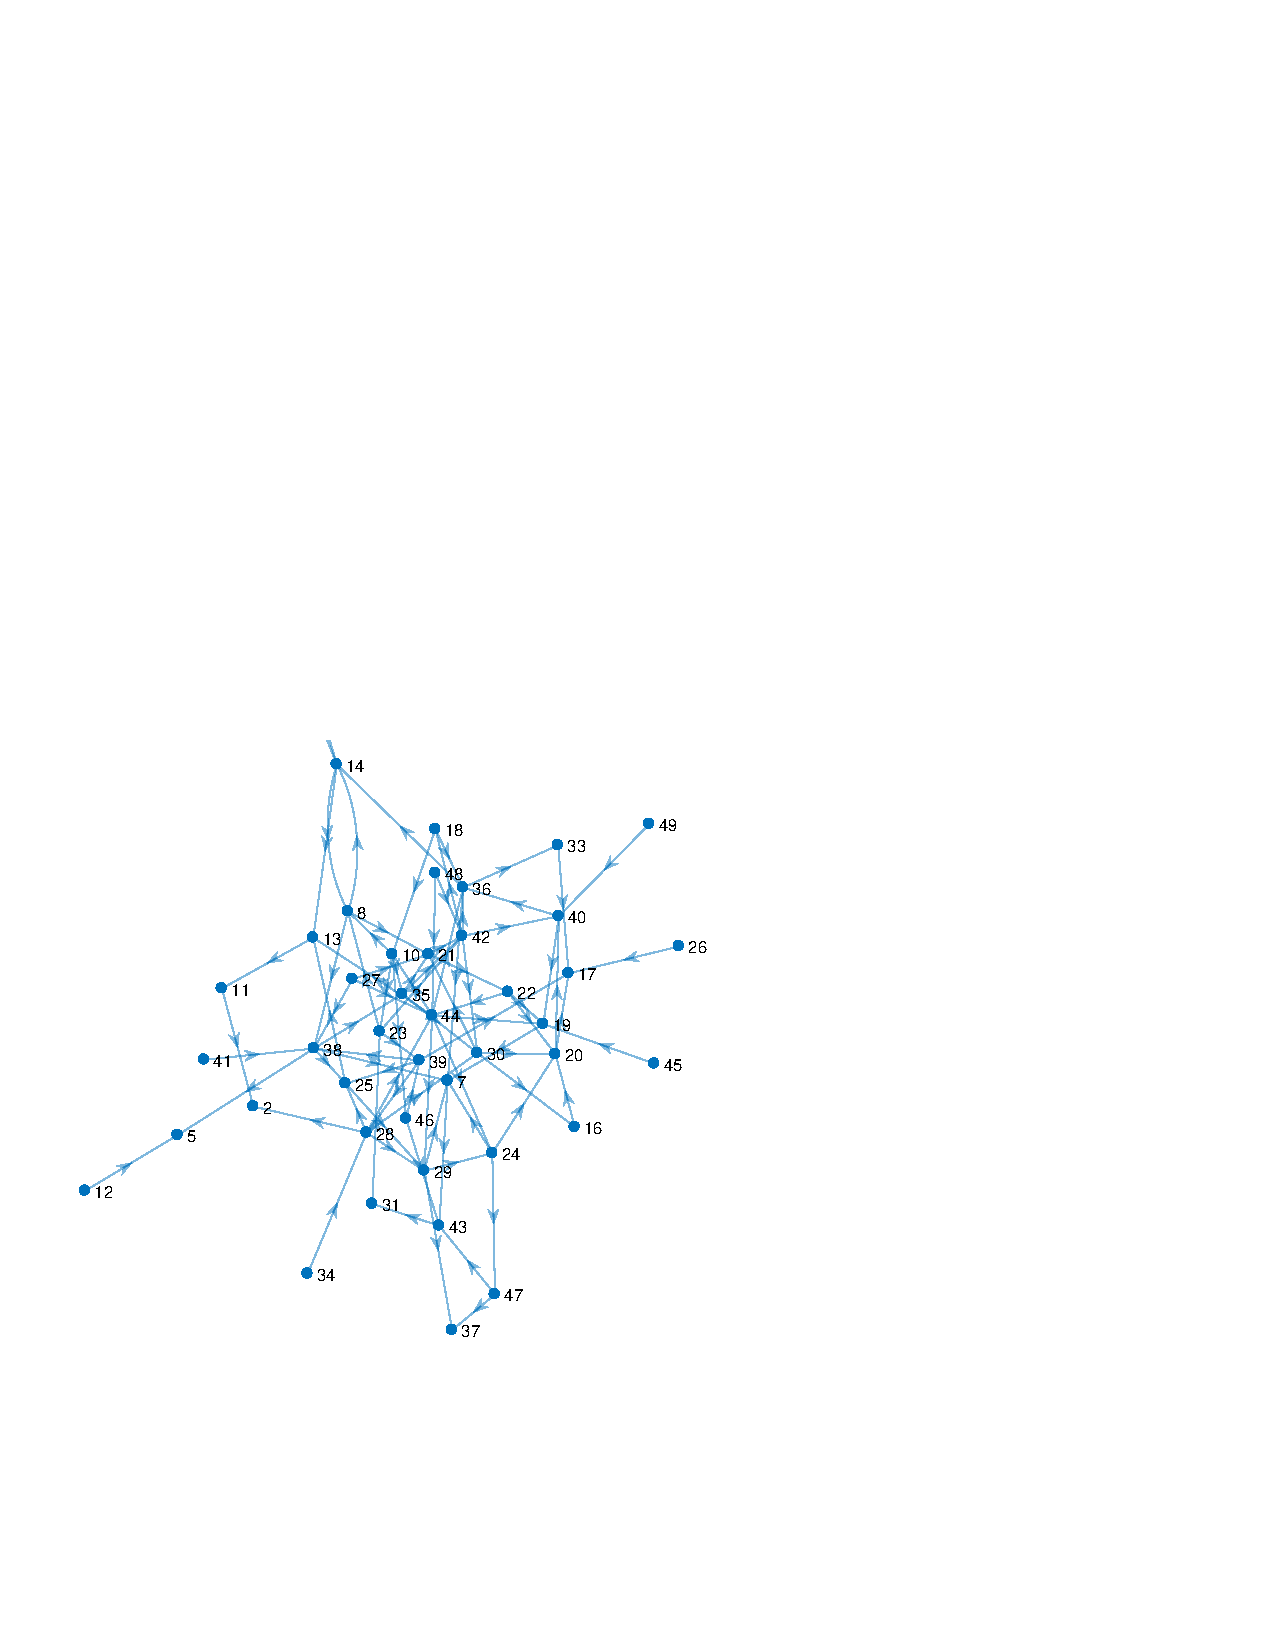
\includegraphics[width=0.8\linewidth]{dag}
\caption{A Directed Acyclic Graph of the Running AUTOSAR Software Application, Runnables = 50, Paths = 35, Activation Patterns shown in Table \ref{tbl_requirements}.}
\label{fig_application}
\end{figure}
\begin{center}
\small
\begin{minipage}{.5\textwidth}%
\centering
\begin{tabular}{@{}p{0.25cm}lll@{}}
\toprule
C& $r_i$ & $(e_{r_im_1}, e_{r_im_2}, e_{r_im_3})$ & $period$\\ \midrule
\multirow{4}{4em}{c1} 
&$r_1$ & (0.030, 0.060, 0.090) & 1\\
&$r_2$ & (0.041, 0.081, 0.122) & 2\\
&$r_3$ & (0.083, 0.167, 0.250)  & 5\\ 
&$r_4$ & (0.310, 0.620, 0.930) & 10 \\[0.3em]
\hline
\multirow{2}{4em}{c2} 
&$r_1$ & (0.310, 0.620, 0.930) & 10\\
&$r_2$ & (0.310, 0.620, 0.930) & 10\\
&$r_3$ & (0.310, 0.620, 0.930)  & 10\\ 
&$r_4$ & (0.310, 0.620, 0.930) & 10 \\[0.3em]
\hline
\multirow{2}{4em}{c3} 
&$r_1$ & (0.310, 0.620, 0.930) & 10\\
&$r_2$ & (0.291, 0.583, 0.874)) & 10\\
&$r_3$ & (0.291, 0.583, 0.874)  & 20\\ 
&$r_4$ & (0.291, 0.583, 0.874) & 20 \\[0.3em]
\hline
\multirow{2}{4em}{c4} 
&$r_1$ & (0.291, 0.583, 0.874) & 20\\
&$r_2$ & (0.291, 0.583, 0.874)) & 10\\
&$r_3$ & (0.291, 0.583, 0.874)  & 20\\ 
&$r_4$ & (0.093, 0.186, 0.279) & 50 \\[0.3em]
\hline
\multirow{2}{4em}{c5} 
&$r_1$ & (0.420, 0.841, 1.261) & 100\\
&$r_2$ & (0.420, 0.841, 1.261)) & 100\\
&$r_3$ & (0.420, 0.841, 1.261)  & 100\\ 
&$r_4$ & (0.420, 0.841, 1.261) & 100 \\[0.3em]
\bottomrule
\end{tabular}
\captionof{table}{Specification of Components.}
\label{tbl_comps_config}
\end{minipage}~
\begin{minipage}{.45\textwidth}
\begin{center}
    \begin{tabular}{@{}lll@{}}
    \toprule
    Activation, $AP$ & Share & Time, ms \\ \midrule
    $\tau_1$ & 50  & 50\\
    $\tau_1\rightarrow\tau_2$ & 20  & 100\\
    $\tau_1\rightarrow\tau_2\rightarrow\tau_3$ & 20  & 200\\
    $\tau_1\rightarrow\tau_2\rightarrow\tau_3\rightarrow\tau_4$ & 10  & 400\\
    \bottomrule
    \end{tabular}
    \captionof{table}{Activation Patters of Cause-effect Chains, their Share and End-to-end Timing Requirements.}
    \label{tbl_requirements}
\end{center}
\begin{center}
    \begin{tabular}{@{}llll@{}}
    \toprule
    M  & $P_{idle}$& $P_{busy}$& $\lambda$ \\ \midrule
    $m_1$ & 50.0& 140.0 &1.0E-3  \\
    $m_2$ & 10.0& 100.0 &1.0E-4  \\
    $m_3$ & 10.0& 140.0 &1 .0E-5 \\ \bottomrule
    \end{tabular}
    \captionof{table}{Computation Nodes Specification.}
    \label{tbl_nodes_specification}
\end{center}
\end{minipage}
\end{center}

In the next subsequent subsections, we propose a metaheuristic approach which is based on Particle Swarm Optimization (PSO) and hybrid PSO. Furthermore, we elaborate the approach using the presented running example.

\section{Integer Linear Programming Approach}
In the ILP approach, we represent the feasible solution $x$ of the allocation problem as a 3-dimensional binary matrix, where $x^k_{ij}$ refers to the allocation of a software component $c^k_i$ on node $m_j$, $c^k$ refers to the $k^{th}$ replica of $c$. For the running example, a particular feasible solution is shown in Figure \ref{fig_matrix_feasible_solution}.


\begin{center}


\begin{equation*}
\textbf{$\textbf{x}$}=
\begin{bmatrix} 

%first element
\begin{minipage}{.3\textwidth}
\centering
\[
\begin{bmatrix} 
x_{11}^1 & x_{12}^1 & \dots & x_{1J}^1\\
x_{21}^1 & x_{22}^1 & \dots & x_{2J}^1\\
\vdots & \vdots & \ddots & \vdots\\
x_{I1}^1 & x_{I2}^1 & \cdots & x_{IJ}^1
\end{bmatrix}
\]
%second element
\end{minipage}~
\begin{minipage}{0.3\textwidth}
\centering
\[
\begin{bmatrix} 
x_{11}^2 & x_{12}^2 & \dots & x_{1J}^2\\
x_{21}^2 & x_{22}^2 & \dots & x_{2J}^2\\
\vdots & \vdots & \ddots & \vdots\\
x_{I1}^2 & x_{I2}^2 & \cdots & x_{IJ}^2
\end{bmatrix}
\]
\end{minipage}
% dots
...
%last element
\begin{minipage}{0.3\textwidth}
\centering
\[
\begin{bmatrix} 
x_{11}^K & x_{12}^K & \dots & x_{1J}^K\\
x_{21}^K & x_{22}^K & \dots & x_{2J}^K\\
\vdots & \vdots & \ddots & \vdots\\
x_{I1}^K & x_{I2}^K & \cdots & x_{IJ}^K
\end{bmatrix}
\]
\end{minipage}

\end{bmatrix}
\end{equation*}

\captionof{figure}{A Feasible Solution $x$ for K=2.}
\label{fig_matrix_feasible_solution}
\end{center}
% \begin{center}
% \begin{minipage}{.4\textwidth}
% \centering
% \begin{equation}
% \textbf{x$^0$}=
% \begin{bmatrix} 
% 0 & 1 & 0\\
% 1 & 0 & 0\\
% 0 & 1 & 0\\
% 0 & 1 & 0\\
% 0 & 1 & 0
% \end{bmatrix}
% \end{equation}
% \end{minipage}~
% \begin{minipage}{0.4\textwidth}
% \centering
% \begin{equation}
% \textbf{x$^1$}=
% \begin{bmatrix} 
% 0 & 0 & 1\\
% 0 & 1 & 0\\
% 0 & 0 & 1\\
% 0 & 0 & 1\\
% 0 & 0 & 1
% \end{bmatrix}
% \end{equation}
% \end{minipage}
% \captionof{figure}{A Feasible Solution $x$ for K=2.}
% \label{fig_matrix_feasible_solution}
% \end{center}

\subsection{Objective Function}
The power consumption $p(x)$ is computed as the sum of the average power consumption of individual nodes $p_m(x)$ by using Equation \ref{eqn_avgpowerconsumption_util}, where $p_m(x)$ is computed first using Equation x, with utilization of the node $u_m$ as its argument, which is calculated using Equation \ref{lbl_util}as the sum of the utilization of the components (including the replicas) allocated to that node. A component's utilization is obtained from the sum of the utilization of the tasks that realize the component's functionality using Equation \ref{eqn_util_component}.

\begin{align}
\label{eqn_avgpowerconsumption_util}
p(x) = \sum\limits_{m\in M}{p_{m}(x)}&\\
\label{lbl_power}
p_{m}(x) = f_p(u_{m}{(x)})&\\
\label{lbl_util}
u_{m}{(x)} = \sum_k{\sum_i{u_{c_i}*x^k_{ij}}} & \text{ where }j=M^{-1}(m)\\
\label{eqn_util_component}
u_c = \sum_{\tau\in T_{c}} \frac{Exec(\tau_{m})}{Period(\tau)}&
\end{align}

Table \ref{tbl_powerconsumption} illustrates the power consumption calculation of the software allocation example for the feasible solution (\ref{fig_matrix_feasible_solution}).

% Please add the following required packages to your document preamble:
% \usepackage{booktabs}
\begin{table}[h]
\linespread{1.0}\small
\centering
\begin{tabular}{@{}llll@{}}
\toprule
M  & C                             					& $U_c (x)$                                    & $P_m (x)$      \\ \midrule
$m_1$ & {[}$c^1_2${]}                     			& {[}0.046, 0.017{]}                       & 61.155W  \\[0.3em]
$m_2$ & {[}$c^1_1, c^2_2, c^1_3, c^1_4, c^1_5${]} 	& {[}0.196, 0.248, 0.149, & 114.648W \\[0.3em]
		& & 0.091, 0.034{]} &\\[0.3em]
$m_3$ & {[}$c^2_1, c^2_3, c^2_4, c^2_5${]}     		& {[}0.224, 0.137, 0.050{]}                & 131.731W \\[0.3em] \bottomrule
& & Total Power Consumption & 307.534W\\
\end{tabular}
\caption{Average and Total Power Consumption of Nodes.}
\label{tbl_powerconsumption}
\end{table}

In the ideal case, the minimum power consumption of the distributed system is achieved by centralizing the application on fewer nodes. However, due to the timing and reliability constraints, which require additional computing resources, the optimal solution could result in more used nodes. 

\subsection{Constraints}
\paragraph{Software Application Reliability Constraint}
An optimal solution $x$ must fulfill the application reliability requirement RelReq, which is usually in the range [$0.999, 0.999999$] for safety-critical applications. The ILP formulation of the application reliability model, which is shown in (\ref{eqn_appreliability}), is shown in (\ref{eqn_appreliability_milp}).
\begin{align}
\label{eqn_appreliability_milp}
Reliability(x)=\sum_{s\in PS}[f(x,s)]*p_s,
\end{align}
where $[f(x,s)]$ is an \textit{Iverson function } that returns $0$ if the proposition that the application functions in state $s$ is \textit{true}. Otherwise it returns $1$ if the proposition that application functions in state $s$ is \textit{false} (or the application fails in state $s$ is \textit{true}). The application functions only if all of its constituent software components functions and fails if at least of one of its components fails as formulated in (\ref{eqn_appreliability_milp_components}), via the floor function. A software component functions if there exists a node $m_j$ that hosts the component's replica $x_{ij}^k=1$ and at the same time the node functions $s_{j}=1$, which is formulated in (\ref{eqn_appreliability_milp_component}) via the ceiling function. The floor and ceiling functions are piecewise linear functions, and are linearized by the ILP solver.

\begin{align}
f(x,s) = \floor[\Bigg]{\frac{\sum_if_{c_i}(x,s)}{N}}=
\begin{cases}
1 & \mbox{if } application \mbox{ functions}\\
0 & \mbox{if } application \mbox{ fails}
\end{cases}\label{eqn_appreliability_milp_components}\\
f_{c_i}(x,s) = \ceil[\Bigg]{\frac{\sum_k\sum_j x^{k}_{ij}*s_j}{K}}=
\begin{cases}
1 & \mbox{if } c_i \mbox{ functions}\\
0 & \mbox{if } c_i \mbox{ fails}
\end{cases}\label{eqn_appreliability_milp_component}
\end{align}

Table \ref{tbl_application_rel} demonstrates the application reliability calculation for the feasible solution $x$ (\ref{fig_matrix_feasible_solution}). %Figure~\ref{fig_comp_replications} shows pictorial descriptions of component allocations on nodes with no replication $K=1$, and with replications $K=2$. 
\begin{table}[h]
\centering
\begin{tabular}{@{}llll@{}}
\toprule
$s$   & $p_s$     & {[}$f_{c_i}(x), i=1,2,3,4${]} & $f_a(x)$ \\ \midrule
000 & 0.0000000000 & {[}0, 0, 0, 0{]}          & 0     \\
001 & 0.0000000099 & {[}0, 0, 0, 1{]}          & 0     \\
010 & 0.0000000099 & {[}1, 1, 1, 1{]}          & 1     \\
011 & 0.0000999800 & {[}1, 1, 1, 1{]}          & 1     \\
100 & 0.0000000099 & {[}1, 1, 1, 0{]}          & 0     \\
101 & 0.0000999800 & {[}1, 1, 1, 0{]}          & 0     \\
110 & 0.0000999800 & {[}1, 1, 1, 1{]}          & 1     \\
111 & 0.9997000299 & {[}1, 1, 1, 1{]}          & 1     \\ \bottomrule
\end{tabular}
\caption{Application Reliability Calculation using State Enumeration Method, R(x) = 0.9998999998.}
\label{tbl_application_rel}
\end{table}

% \begin{figure}
%     \centering
%     \begin{subfigure}[b]{0.2\textwidth}
%         \includegraphics[width=\textwidth]{k0}
%         \caption{No replication, K = 1.}
%         \label{fig:datachainsingle}
%     \end{subfigure}
%     ~ %add desired spacing between images, e. g. ~, \quad, \qquad, \hfill etc. 
%       %(or a blank line to force the subfigure onto a new line)
%     \begin{subfigure}[b]{0.25\textwidth}
%         \includegraphics[width=\textwidth]{k1}
%         \caption{With replication, K = 2.}
%         \label{fig:datachainmulti}
%     \end{subfigure}
% %     ~
% %         \begin{subfigure}[b]{0.3\textwidth}
% %         \includegraphics[width=\textwidth]{k2}
% %         \caption{With Replication, K = 3}
% %         \label{fig:datachainsingle}
% %     \end{subfigure}
%     \caption{Allocation of Components.}
%     \label{fig_comp_replications}
% \end{figure}

In the case that the application reliability could be met with less replications, there is no need to keep unnecessary component replicas in the system. To this end, our optimization algorithm imposes soft constraints for $k>1$, which implies that replicas allocated on the same node are reduced to a single replica, essentially discarding the extra replicas by design, since the reliability does not improve following additional replicas on the same node, assuming our fault model.

\paragraph{Timing Constraints}
The timing constraints ensure that the response times of the tasks realizing the distributed application meet their deadlines. Furthermore, they ensure that the cause-effect chains satisfy their respective end-to-end timing requirements, for all possible failure-modes of the system. The constraints are formulated as logical constraints in the ILP problem, as explained in the rest of this subsection.

\paragraph*{Tasks Deadline Constraints}
The following pseudo-code illustrates how the ILP logical constraints of the tasks deadlines are prepared. It explores all possible sets of components combinations (or partitions) that can potentially be allocated to a node. Only the sets that are schedulable are asserted as constraints of the optimization problem, which is explained as follows: Line (1) identifies the power set of the components $Par$, followed by synthesis of tasks models of each partition. Line (2) checks the tasks models' schedulability and returns a matrix $M^T$ that indicates schedulability, which is \textit{true} if the task model is schedulable and \textit{false} if not schedulable. Line (3) generates an ILP partition expression $E$ for each node, then Line (4-6) asserts the expressions to hold in the optimization for the partitions that are schedulable.
\begin{algorithm}
\SetKwData{Particles}{Particles}
\SetKwInOut{Input}{input}\SetKwInOut{Output}{output}
\SetKwFunction{AssertOR}{assertOR}
\caption{Generate Task Partitions Constraints.}\label{alg_partition}
% \algsetup{
% linenosize=\small,
% linenodelimiter=.
% }	
%\renewcommand{\algorithmicrequire}{\textbf{Input:}}
%\renewcommand{\algorithmicensure}{\textbf{Output:}}
%\begin{algorithmic}[1]
\Input{$C,M$}
\Output{Optimization Satisfies Tasks Deadlines, $D$}
$Par \Leftarrow 2^C$\;	
$M^T\Leftarrow isSched(Par, M)$\;
$E\Leftarrow MilpParExp(x)$\;
\ForEach{$m \in M$}{
	\AssertOR{$M^T_m, E_m, true$}
}
\end{algorithm}

In general, the number of potential logical constraints grow exponentially, which is in $2^{|C|}*|M|$. However, the effective logical constraints that are eventually asserted are much lower, for two main reasons: 1) a portion of the tasks models are not schedulable, therefore eliminated from the power set, due to CPU utilization exceeding the bound, hence not satisfying the response time of either task in the partition; ii) a task model can be a super set of other tasks model. In this case, only the super model is checked, hence reducing pre-optimization time and logical constraints asserted in the solver.

\subsubsection*{Cause-effect Chains Constraints}
These constraints ensure that the cause-effect chains $\Gamma$ meet their respective end-to-end requirements $\mathrm{E2eReq}$. Similar to the previous constraints, the cause-effect chain constraints are logical assertions, which must be fulfilled by the optimal solution. The following pseudo-code illustrates how the ILP logical assertions are synthesized from the input models. 
The pseudo-code contains three main parts: i) the first part in Line (2) identifies the different deployment cases of the cause-effect chains over a set of nodes $M$, ii) the second part in Line (3-5), checks the schedulability of a deployable cause-effect chain $\phi$ against the reaction or age delays  \cite{mubeen2013support} and returns its schedulability matrix $M^\Gamma$, with values $true$ if schedulable and $false$ if not schedulable. For a schedulable $\phi$, Line (5) constructs a conjunctive ILP expression that indicates the existence of at least one schedulable $\phi$ that satisfies the end-to-end requirement imposed on $\gamma$, and iii) the last part in Line (7) asserts the ILP logical OR expressions for each $\gamma$.
\begin{algorithm}
\SetKwData{Particles}{Particles}
\SetKwInOut{Input}{input}
\SetKwInOut{Output}{output}
\caption{Generate Constraints on the Cause-effect Chains.}\label{alg_causeeffectchains}
%\begin{algorithmic}[1]
\Input{$\Gamma,M$}
\Output {Optimization Satisfies End-to-end Requirements of Cause-effect Chains}
\ForEach{$\gamma \in \Gamma$}{
    $\Phi\leftarrow Unique(C^{T_\Gamma}_r, M)$ \;
	\ForEach{$\phi \in \Phi$}{
        $M^\Gamma\Leftarrow isSched(\phi, M)$\;
        $depExp\Leftarrow depExp \lor sched(M^\Gamma, true)$\;
    }
	$assert(depExp)$\;
}
%\end{algorithmic}
\end{algorithm}\vspace{-0.2cm}

\subsection{Solving the ILP Problem}
We use IBM ILOG CPLEX Optimizer to solve our proposed ILP model. CPLEX Optimizer is one of the most robust and high-performing linear programming, mixed integer, and quadratic programming solvers in the market. The ILP problem is encoded in Java via the 

\section{Metaheuristic Approach}
Although the proposed ILP approach provides exact solutions, that is with an AUTOSAR software allocation with minimum power consumption, the approach approach does not scale well for large applications. Thus, in this section, we propose an approximation approach based on several metaheuristic techniques to address the scalability challenge. Metaheuristic techniques assumes little of the problem in question, and therefore are ideal to solve high dimensional and complex optimization problems, that is, problems that are difficult or practically impossible to solve by exact methods, e.g., linear programming, or heuristic techniques, e.g., local search algorithms. They have improved over the last decades with respect to effectiveness, efficiency, and ease of use by providing fewer user-configurable parameters. Metaheuristic techniques do not guarantee optimal solutions, nevertheless, the returned solutions can be good enough (or acceptable) in the eyes of the system designer, for this particular problem, it means although the power consumption of the system is not optimal, the solution can be deemed acceptable, that is as long as the the constraints are fulfilled. In the opposite case, where the constraints could not be fulfilled, the algorithms can be rerun several times until the desired results are found, or the design can be relaxed by weakening the timing and reliability constraints of the system.

Metaheuristic techniques perform differently for different problem types, size, and complexity. In this section, we show application of different metaheuristic techniques that employ swarm intelligence and evolutionary approaches in finding the (near) optimal solutions. Specifically, we apply the Particle Swarm Intelligent (PSO), Differential Evolution techniques primarily, and further hybrid PSO with DE and Hill-climbing for improved performance. PSO has been applied to solve a wide range of problems, including a task allocation problem \cite{yin2007task}, and DE is shown to scale well for problems with high dimensions. In fact, PSO and DE are used together for improved performance in several optimization problems, likewise, PSO is used with local search techniques such as Hill climbing to intensify the search. Finally, we evaluate the different metaheuristic methods based on solution quality and allocation (or computation) time for different software allocation problems.

\subsection{Solution Representation}
In contrast to the \textit{0-1} representation, the integer-linear representation uses much lower number of variables, that is $N*K(L-1)$, e.g., for a software allocation problem with $N=10,L=8,K=2$, 140 variables are saved. Of course the possible values in the former representation is two whereas in the latter representation, it is $L$, which is usually higher and results larger solution space. Nevertheless, the integer-linear representation is compact and computationally more efficient.

\subsection{Fitness Function Definition}
% Define the fitness function
Since a metaheuristic method functions over the meta of a problem, the quality of candidate solutions is evaluated based on their fitness to meet the problem's objective. A solution that delivers lower power consumption and violates less constraints is indicated by a lower fitness value. The fitness function $f(\textbf{x})$ combines the original objective function $P(\textbf{x})$ and the constraints $Timing(\textbf{x}),Reliability(\textbf{x})$ in order to compute real-valued numbers that indicate quality of the candidate solutions.

Consequently, the original constrained optimization problem is transformed into unconstrained optimization problem, by extending the objective function $P(\textbf{x})$ with the constrains, represented by a \textit{penalty function} $\Phi(\textbf{x})$. The function returns 0 if no constrains are violated otherwise returns a positive number, essentially to penalize the candidate solution by increasing its fitness (for our minimization problem), thus discriminating the solution. The function is a combination of $\beta\sum{g_i(\textbf{x})}$ and $\gamma h(\textbf{x})$ functions, respectively computes the timing violations and a software application reliability violation, and each function is weighted to indicate the size of the penalty separately. Moreover, the penalty function $\Phi({\textbf{x}})$ is weighted to indicate the size of penalty that imposed on the combined violations of timing and reliability. \textbf{How to compute the parameters [Hamid]}
\begin{align}
\label{}
    \min_{\textbf{x}\in X}\;\;& f(\textbf{x})=P(\textbf{x}) + \alpha \Phi(\textbf{x})\\
    \label{eqn_penalityfunc}\Phi(\textbf{x}) &= \sum\phi_i(\textbf{x})
\end{align}

\subsection{Penality Function}

\subsection{Metaheuristic Algorithms}
\subsubsection{Particle Swarm Optimization}
% What is PSO
PSO is a population-based technique proposed by Eberhart and Kennedy in 1995 to study social behavior, as inspired by natural swarm intelligence observed from the flocking of birds and schooling of fishes \cite{Kennedy1995ParticleOptimization}. Since then, it is extended in order to address various metaheuristic optimization challenges, such as intensification, diversification, convergence analysis, local optima, parameter tuning, computation time, etc. It is successfully applied on several complex real-world problems, e.g., diagnosis and classification of diseases, efficient engineering designs, tuning control design parameters, scheduling problems, etc \cite{Poli2008AnApplications}. 

In PSO, the population (or swarm) $PN=\{p_1,p_2,…,p_N\}$ is a collection of particles $p_i\in PN$, organized according to a certain population topology \cite{Liu2016TopologyOptimization}. A particle has a position $\textbf{x}$ and a velocity $\textbf{v}$, which denote current location and direction of the particle's motion, and current momentum, respectively. It is a memory-based technique, that is, it remembers the best performance of every particle as well as the best performance of the swarm $\textbf{z}$ in order to plan for the next move of the particles, where $\textbf{y},\textbf{z}$ are position vectors and have the same dimensions as $\textbf{x}$. The velocity of a particle is the resultant vector of its current velocity and the particles attraction vectors $(\textbf{y}-\textbf{x}), (\textbf{z}-\textbf{x})$, respectively, known as \textit{cognitive} and \textit{social} components of the  particle's velocity formula, as shown in Equation \ref{eqn_pso_velocity}. The attraction vectors impose force of attraction on the particle to move closer to their respective components. Thus, the next position of a particle is the resultant of its current position and its next velocity as shown in Equation (\ref{eqn_pso_position}).
\begin{align}
    \label{eqn_pso_velocity}
    \textbf{v} &\leftarrow  \omega\textbf{v} + c_1Rand()\circ(\textbf{z}-\textbf{x}) + c_2Rand()\circ(\textbf{z}-\textbf{x})\\
    \label{eqn_pso_position}
    \textbf{x} &\leftarrow \textbf{x} + \textbf{v}
\end{align}
where $\omega$ is the weight of the velocity, also known as \textit{inertia coefficient}, and controls the convergence of the algorithm, $c_1, c_2$ are acceleration coefficients and controls the weight of attraction towards the cognitive and social components, respectively, $Rand()\in U(0,1)$ is a random function, along the acceleration coefficients, is element-wise multiplied with the components to improve diversity of the search by introducing stochastic behavior.

Although PSO was originally proposed for continuous problem, it is applied to discrete problems successfully as well. In the latter case, the solutions are represented by \textit{0-1} integer variables \cite{KennedyAAlgorithm} or integer-linear by approximation to the nearest integer values \cite{Clerc2000DiscreteProblem}, which is the representation employed adopted in our problem as it is compact, hence fewer decision variables. Accordingly, after the new position (or candidate solution) is determined, following Equations \ref{eqn_pso_velocity} and \ref{eqn_pso_position}, the solution is discretized by rounding off the its elements to the nearest integer values, that is $\textbf{x}\leftarrow [\textbf{x}]$.



% Show the representation of the a solution
% Demonstrated it on the example
% \begin{algorithm}
% \caption{PSO Algorithm}\label{alg_pso}
% \begin{algorithmic}[1]
% \Require n
% \Ensure Near (Optimal) Solution
% \State $x_{sb}\leftarrow$ getWorstPosition()
% \State $Particles\leftarrow$ createParticles($n$)
% \State initParticles($Particles$)
% \While{$!stoppingCritera$}
%     % Calculate personal best, swarm best positions
%     \State \Comment{Calculate personal best and swarm best positions of the particles}
%     \ForAll{$p \in Particles$}
%         \State $particle \leftarrow$  getPosition($p$)
%         \State $x_{pb} \leftarrow$  getPosition($p$) 
%         \If{$fitness(x)\leq fitness(x_{pb})$} \Comment{Personal best position}
%             \State $x_{pb}\leftarrow x$
%             \If{$fitness(x)\leq fitness(x_{sb})$} \Comment{Swarm best position}
%                 \State $x_{sb}\leftarrow x$
%             \EndIf 
%         \EndIf 
%     \EndFor
%     % Calculate next positions of the particles
%     \State \Comment{Calculate next positions of the particles}
% 	\ForAll{$p \in Particles$}
%         \State $v\leftarrow v+c1*r1*(x_{pb}-x)+c2*r2*(x_{sb}-x)$ 
%         \State $x\leftarrow$ getPosition($p$)$ + v$
%         %\State setParticlePosition($p,x$)
%     \EndFor
% \EndWhile
% \end{algorithmic}
% \end{algorithm}\vspace{-0.2cm}

\subsubsection{Differential Evolution}
Similar to PSO, Differential Evolution (DE) is a population-based metaheuristic technique for the global optimization which includes non-linear and non-differentiable problems. It was initially proposed by Storn and Price in 19995 \cite{Storn1997DifferentialSpaces}, since then it has improved with regard to the different operators of DE such as mutation and crossover, and variants over population topology and hybridization \cite{Das2016RecentSurvey}. It is a parallel search technique, therefore, is ideal for computationally intensive problems, and employs mutation and crossover operators that allow the search to skip local minima as opposed to PSO.

In every generation, the population undergoes mutation, crossover, and selection according to the formulas shown in Equation , (\ref{eqn_de_crossover}), and (\ref{eqn_de_selection}), respectively. A mutant vector $v$ is created from randomly selected elements $\{a,b,c\}\in PN$ according the mutation operation shown in Equation (\ref{eqn_de_mutation}), that is by adding the base matrix to the weighted difference matrix $F\circ(b-c)$, where $F$ controls the amplification of the $(\textbf{b}-\textbf{c})$ variation.
\begin{align}
    \label{eqn_de_mutation}
    \textbf{v} & \leftarrow   \textbf{a} + F\circ(\textbf{b}-\textbf{c})\\
    \label{eqn_de_crossover}
    u_{ik} & \leftarrow 
    \begin{cases}
    v_{ik} & \mbox{if } U(0,1) \leq CF \mbox{ and } h = (i*K+k)\\
    x_{ik} & \mbox{if } U(0,1) > CF \mbox{ and } h \neq (i*K+j)
    \end{cases}\\
    \label{eqn_de_selection}
    \textbf{x} &\leftarrow 
    \begin{cases}
    \textbf{u} & \mbox{if } f(\textbf{u}) < f(\textbf{x})\mbox{ functions}\\
    \textbf{x} & \mbox{otherwise }
    \end{cases}
\end{align}

\subsubsection{Hybrid Particle Swarm Optimization}
The canonical PSO technique uses the constriction factors to balance exploitation and exploration of the search space, that is to deliver better quality solutions. Nevertheless, it still suffers from local minima especially for complex and large problems that exhibit especially multimodal behavior. Hybridization of PSO is one the most widely studied approach in the improvement of the the PSO technique. Basically, it combines other optimization techniques, for instance to intensify local search, and improve diversification by introducing stochastic search. However, hybridization of PSO usually incurs additional computation time. Therefore, the benefit of hybridization has to be studied carefully in conjunction to computation time. Moreover, it should not complicate the user-configurable parameters, to be inline with the philosophy of PSO for ease-of-use.

PSO is hybridized with several optimization techniques, such as Genetic Algorithm (GA), DE, local searches (e.g., Hill-climbing, gradient decent, etc.), ant colony, simulated annealing, etc. Of which, it is shown to perform better when hybridized with DE on constrained, discrete, large benchmarks. Furthermore, it is shown to perform better when hybridized with Hill-climbing (specifically \textit{Steepest-descent} variant)for software allocation problem \cite{} in particular. In this paper, we hybridize PSO with DE (DEPSO) and Hill-climbing (HCPSO) to the solve the software allocation problem as formulated in Equation (x). In the latter case, we also apply the stochastic variant of Hill-climbing (SHPSO) in order to offset stagnation of the steepest Hill-climbing when applied on large software allocation problems.

\IncMargin{1em}
\begin{algorithm}[H]
\SetKwData{P}{P}\SetKwData{S}{sBest}
\SetKwData{Generation}{Generation}
\SetKwData{Interval}{Interval}
\SetKwData{Particles}{Particles}
\SetKwInOut{Input}{input}\SetKwInOut{Output}{output}
\SetKwFunction{OptimizeUsingDE}{optimizeUsingDE}
\SetKwFunction{OptimizeUsingHC}{optimizeUsingHC}
\SetKwFunction{OptimizeUsingSHC}{optimizeUsingSHC}
\SetKwFunction{ComputeParticleVelocity}{computeParticleVelocity}
\SetKwFunction{ComputeParticlePosition}{computeParticlePosition}
\SetKwFunction{InitPSO}{initPSO}

\BlankLine
\Input{PSO parameters, DE parameters}
\Output{Software allocation solution \S .\textbf{x}}
\BlankLine
\Particles $P$ $\leftarrow$ \InitPSO{}\;
\BlankLine
 \While{termination criteria}{
  $P$ $\leftarrow$\ComputePersonalBest{$P$}\;
  \S $\leftarrow$\ComputeSwarmBest{$P$}\;
  \BlankLine
   \ForEach{$p\in P$}{
        \ComputeParticleVelocity{$p$} according to Equation (\ref{eqn_pso_velocity})\;
        \ComputeParticlePosition{$p$} according to Equation (\ref{eqn_pso_position})\;
   }
   \If{interval criteria}{
        $P$ $\leftarrow$ \OptimizeUsingDE{$P$}\;
    \tcp{$P$ $\leftarrow$ \OptimizeUsingHC{$P$}}\label{hc}
    \tcp{$P$ $\leftarrow$ \OptimizeUsingSHC{$P$}}\label{sh}
   }
 }
 \caption{Hybrid PSO Algorithms.}\label{alg_depso}
\end{algorithm}\DecMargin{1em}
 
\subsubsection{Differential Evolution PSO (DEPSO)}
DE complements the classical PSO by introducing stochastic behavior via the evolutionary operators such as mutation, cross-over and selection. In this specific hybridization approach, we allow the DE algorithm to run intermittently for some number of generations before the next PSO generation starts.

\subsubsection{Hill-climbing PSO}
Hill-climbing is a popular local search based on the notion of \textit{neighborhood}, that is, the candidate solution (or neighbor) that performs better is selected iteratively until no improvements can be made. The software allocation solution $\textbf{x}$ is neighbor to $\textbf{x\textquotesingle}$ if $\textbf{x}=\textbf{x\textquotesingle}$ except $\exists i,j|\;x_{ij}\neq x\textquotesingle_{ij}$, that is, a single mapping is different. In every iteration, the best neighbor is selected, and subsequently replaces the current candidate solution if it performs better, and continues until maximum iteration, this variant is known as Steepest-descent Hill-climbing (SHC).

Since SHC exhaustively checks all neighbors before moving to the next iteration, the computation time is high especially for high-dimensional problems. To offset this problem, we also apply the stochastic version of Hill-climbing. In the later case, the neighbor is selected randomly, first by selecting the dimension, that is the component $c_{ij}$, where $i=U(1,I)$ and $j=U(1,K)$, second, selecting the value, that is the node $n_j$, where $j=U(1,J)$. If the neighbor improves the current candidate solution sufficiently, the search moves to the next iteration, which is until no more improvements can be made.


\begin{figure*}
    \centering
    \begin{subfigure}[b]{0.4  \textwidth}
        \includegraphics[width=\textwidth]{util}
        \caption{Utilization of Nodes.}
        \label{fig_util}
    \end{subfigure}
    ~%\hspace{-0.4cm}
        \begin{subfigure}[b]{0.4\textwidth}
        \includegraphics[width=\textwidth]{power}
        \caption{Power Consumption of Nodes.}
        \label{fig_power}
    \end{subfigure}
    \caption{Allocation of Applications on Heterogeneous Nodes.}
    \label{fig_util_power}\vspace{-0.2cm}
\end{figure*}
\section{Evaluation}\label{sec_evaluation}
In this section, we evaluate the proposed approach using  synthesized automotive applications that conform  to the automotive benchmark proposed by Kramel et al.~\cite{Kramer2015RealFree}. The number of runnables, timing specification and activation patterns within the cause-effect chains are also selected according to the benchmark. In order to show the scalability of our approach and to assess the scope of its applicability in practice, in some cases, we use higher specifications standard  than what is indicated in the benchmark, e.g., the maximum number of activation patterns is extended from three to four.

In the rest of the section, we describe the setup and method of evaluation, followed by discussion of the evaluation results.

%\subsection{Preparation}
\subsection{Evaluation Setup}
The evaluation setup consists of three hardware platforms with different computing capacities, i.e., processing speed and memory size as shown in Table~\ref{tbl_hardwaremodel}. The evaluation on different platforms can be used as performance indicator and also to identify performance bottlenecks in the model. HP EliteBook and Lenovo 20378 are personal computers with core-i5 and core-i7 processors, respectively, whereas PowerEdge is a workstation with much higher processing and memory specification than the personal computers.
\begin{table}[h]
\centering\small
\begin{tabular}{@{}p{0.25\columnwidth}p{0.275\columnwidth}llll@{}}
\toprule
Hardware Model  & Pro. Model & \rotatebox{70}{\#Pro.} & \rotatebox{70}{\#Core} & \rotatebox{70}{Cache} & \rotatebox{70}{RAM}\\ \midrule
$^1$HP EliteBook & $^3$Core i5, 2.2GHz & 1 & 2 & 3M & 8G \\ 
Lenovo 20378 & $^4$Core i7, 2.6GHz & 1 & 4 & 6M & 16G\\ 
$^2$PowerEdge & $^5$Xeon(R), 2.4GHz & 24 & 6 & 15M & 256G\\
\bottomrule
\end{tabular}
\caption{Summary of the Hardware Specifications.\\
\footnotesize{$^1$HP EliteBook 840 G2, $^2$PowerEdge R730 Rack Server}\\
\footnotesize{$^3$Intel® Core™ i7-4720HQ @ 2.60GHz, $^4$Intel® Core™ i7-4720HQ @ 2.60GHz $^5$Intel(R) Xeon(R) CPU E5-2620 v3 @ 2.40GHz}}
\label{tbl_hardwaremodel}
\end{table}

\subsubsection{Software Application Specification} In order to evaluate the proposed approach on different ranges of applications, we automatically generate synthetic examples that comply with the automotive benchmark~\cite{Kramer2015RealFree}. The examples denote simple to complex automotive functions such as reverse-parking assistance system and engine control system. For simplicity, we identify three classes of applications with different sizes and complexity, shown as tuple $(c, r, t, g)$, respectively for the number of software components, runnables, tasks, and cause-effect chains. Table \ref{tbl_appsspec} shows the range of values used in the applications for evaluation. 
\begin{table}[h]
\centering\small
\begin{tabular}{@{}llll@{}}
\toprule
Parameter  		& Spec.-I  & spec.-II & spec.-III\\ 
\midrule
components, $c$		& $\leq 10$	& $\leq 15$ 	& $> 15$\\ 
runnables, $r$		& $\leq 50$	& $\leq 100$ 	& $> 100$\\
tasks, $t$ 			& $\leq 30$ & $\leq 60$ 	& $> 60$\\
cause-effect chains, $g$ & $\leq$ 30 & $\leq$ 40 & $> 60$\\ \midrule
activation-pattern	& \multicolumn{3}{c}{$[2,3,4]$}\\ \midrule
share of activation-patterns	& \multicolumn{3}{c}{$[0.7, 0.2, 0.1]$}\\
\bottomrule
\end{tabular}
\caption{Specification of the Applications for Evaluation.}
\label{tbl_appsspec}
\end{table}

\subsubsection{Platform Specification} The specification of nodes can be obtained from simulation, vendor product specification and  experience. Figure~\ref{tbl_nodesspecs} shows the range of values that are used in the nodes' specification. In the experiment, the values are randomly generated while respecting the benchmark.
\begin{table}[h]
\centering\small
\begin{tabular}{@{}llll@{}}
\toprule
Parameter  		& Range\\ 
\midrule
nodes							& $4-10$\\
power consumption (Watt), $p$ 	& $10 - 200$\\
failure-rate (/Mhr), $\lambda$ 	& $10^4 - 10^{-2}$\\
speed factor, $hz$			 	& $0.0 - 1.0$\\
\bottomrule
\end{tabular}
\caption{Range of Values for the Specification of Nodes.}
\label{tbl_nodesspecs}
\end{table}

\subsubsection{Method of Evaluation}
We conduct three experiments that assess the proposed approach for scalability in terms of \textit{allocation time}. The allocation time is defined as the time required to prepare and solve the allocation problem using the proposed ILP method. Furthermore, we show resource efficiency in terms of saving nodes (i.e., using smaller number of nodes). The experiments consist of: i) varying the size of applications in order to observe the effect of increasing components, runnables and tasks in the system, ii) varying the complexity of applications in order to observe the effect of cause-effect chains in the system, and iii) varying the replications. The experiments are discussed in detail in the next subsection.

A preliminary analysis of the evaluation indicates a successful termination of the allocation for Spec-I\&II of the applications. Whereas for Spec-III, the allocation problem is intractable. In fact, it took days on the PowerEdge machine and many times it did not terminate successfully. Therefore, the experimental results that are shown in this paper are conducted on the Spec-I\&II classes. 
\begin{figure}[t!]
\centering
\includegraphics[width=1\linewidth]{increasing_components}
\caption{Effect of Varying the Application Size on the Allocation Time and Number of Utilized Nodes.}
\label{fig_increasing_components}
\end{figure}

\subsection{Varying the Size of Application} 
This refers to increasing the number of software components, as well as runnables, tasks, and cause-effect chains in the system. Figure~\ref{fig_increasing_components} shows the effect of increasing the size of an application from $(c4,r40,t19,g30)$ to $(c10,r100,t57,g60)$ on the allocation time and  the number of nodes utilized. The applications are allocated to a pool of 8 heterogeneous nodes sharing a single network and with specifications shown in Table~\ref{tbl_nodesspecs_exp}. The specifications are generated randomly, with uniform distribution, within the scope of Table~\ref{tbl_nodesspecs}.
\begin{table}
\centering\small
\setlength{\tabcolsep}{4pt}
\begin{tabular}{@{}lllllllll@{}}
\toprule
Node  		& m1 & m2 & m3 & m4&m5&m6&m7&m8\\ 
\midrule
$P_{min}$ & 10 	& 40 	&	30 	&	20 	& 30 	& 	40	&	20&	10\\
$P_{max}$ & 80	& 120	&	120	&	170	&	140	&	130	&	140 &110\\
$\lambda$  &$10^{-3}$	&$10^{-3}$	&$10^{-4}$&$10^{-5}$&$10^{-6}$&$10^{-2}$&$10^{-6}$&$10^{-4}$\\
\bottomrule
\end{tabular}
\caption{Specification of Nodes.}
\label{tbl_nodesspecs_exp}\vspace{-0.4cm}
\end{table}

The CPLEX solver returns an optimal solution for the application $(c8, r80,t44,g30)$ within 6.06 sec. The allocation time increased sharply to 30.3 sec and 129.4 sec respectively for 9 and 10 components. Even if not indicated in this chart, the solver, the solver returns an optimal solution within 45 min for components reaching 15 on the PowerEdge machine and OutOfMemory error on the Lenovo and HP machines. Figure~\ref{fig_util} and Figure~\ref{fig_power} show the utilization and power consumption on each node for the different application sizes. The optimal allocation, in the general case, favor nodes with higher processor speed and lower power consumption specifications.

\subsection{Varying the Number of Cause-effect Chains} 
In order to observe the effect of increasing the cause-effect chains on the allocation time, we vary the number of chains in the application from 10 to 60, which is consistent with the benchmark~\cite{Kramer2015RealFree}. The share of activation patterns also increases proportionally with the ratio $1:[0.7, 0.2, 0.1]$, respectively, for two, three, and four activation patterns. For instance, out of 10 cause-effect chains, there are 7 chains (with two activation patterns), 3 chains (with three activation patterns), and 1 chain (with four activation patterns). The experiment is conducted on two cases of schedulability analysis, namely response time analysis (RTA) and utilization bound (UB), and their result is shown in  Figure~\ref{chart_cause_effect_chain} for increasing number of chains.
\begin{figure}[h!]
\centering
\includegraphics[width=1\linewidth]{increasing_cause-effect_chains}
\caption{Effect of Increasing Cause-effect Chains (under RTA and UB) on the Allocation Time.}
\label{chart_cause_effect_chain}\vspace{-0.4cm}
\end{figure}

The figures in the data table show an exponential growth of allocation time whenever the cause-effect chains are increased linearly for a specific application, in both cases of schedulability analysis. In the case of RTA, the overhead in the pre-optimization is higher than the overhead in the optimization for 50 or less chains. Whereas in the UB case, the computational time of pre-optimization is almost always less than the computational time of the optimization. 
The results are consistent with our expectation that the RTA computation, in the preparation of the timing assertions, is expensive, albeit provides schedulable tasks allocation based on the fixed-priority scheduling policy. In contrast, the UB computation time is relatively low; however, the search space gets larger due to more and more feasible tasks partitioning and chains fulfilling the timing constraints. As a result, the optimization time in the case of UB is usually higher as compared to the case of RTA. Therefore, for applications with chains not more than 40 and naive scheduling assumption using UB, the experiments favor the UB assumption. Whereas, the allocation with the RTA assumption should be selected for applications with exact scheduling requirements. Note, the scalability of this experiment should be seen in conjunction with the experiment discussed in the previous subsection.

\subsection{Varying Replications}
In this experiment, we evaluate the allocation time of the applications with the increase in the number of replications. For the applications specification shown in Figure \ref{fig_replication}, we vary the replications from 1 to 4. 
The allocation in all applications took not more than 10 sec for replications 1 and 2. For Spec-I with replication 3 and 4, the allocation time went up close to 1 min. For Spec-III with replication 3, the allocation time went up rapidly to 30 min, and took extremely large time for replication 4 which is also the case for Application-II.
\begin{figure*}[h]
    \centering
    \begin{subfigure}[b]{0.475\textwidth}
        \includegraphics[width=\textwidth]{replications}
        \caption{Effect on Allocation Time.}
        \label{fig_replication_1}
    \end{subfigure}
    ~
        \begin{subfigure}[b]{0.475\textwidth}
        \includegraphics[width=\textwidth]{replication_comparison}
        \caption{Effect on Pre-optimization.}
        \label{fig_replication_2}
    \end{subfigure}
    \caption{Effect of Varying the Component Replications on the Allocation Time.}
    \label{fig_replication}\vspace{-0.5cm}
\end{figure*}

Figure~\ref{fig_replication_2} shows the effect of shared constraints on the overhead of replications during the pre-optimization and optimization phases of the allocation. In the pre-optimization phase, the allocation time was stable for the increased size of applications. This is due to the fixed constraints regardless of the replications. In contrast, the allocation time increases during optimization as the constraints are applied for the various combination of task partitions, cause-effect chains, and reliability states generated as the result of replications.

\section{Related Work}\label{sec_RW}
%There are a large number of research works analyzing the reliability of distributed systems with a focus on hardware faults (computing and communication equipment errors). In other words, they assume that the software part of the system is perfect and the source of unreliability of the system is hardware faults ~\cite{dai2003study}\cite{zhang2015maximizing}\cite{faragardi2013analytical}.

In a heterogeneous distributed systems where computing nodes and communications links could have various hazard rates, a reliability-aware allocation of tasks to nodes, and using the links with the lowest hazard rates can noticeably improve the system reliability~\cite{shatz1992task}\cite{kartik1997task}\cite{yin2007task}\cite{zhang2015maximizing}. 
%This approach has been used in multiple works to improve the system reliability with no extra hardware/software cost~\cite{yin2007task}\cite{zhang2015maximizing}. 
Interleaving real-time constraints into the problem adds more complexity to reliability-aware task allocation in distributed systems~\cite{faragardi2013optimal}. As opposed to \cite{Wozniak2013AnArchitectures}\cite{Saidi2015AnArchitectures}, we assume that software applications are multi-rate, i.e., the applications execute with different period (or activation patterns). Multi-rate applications increase the difficulty of software allocation due to the several timed paths traversing from the source to the sink in cause-effect chains.

Although improving reliability of the system using a reliability-aware task allocation does not impose extra hardware/software cost,  in reliability-based design approach, redundancy (or replication) of software or hardware components is frequently applied to improve reliability. In such systems not only optimal allocation of software components (or replicas) should be taken into account but also the cardinality of the replicas should be limited for improved efficiency while meeting the desired reliability requirement. The integration of these two approaches (i.e., reliability-aware task allocation and application redundancy) is a promising technique to deal with high criticality of the system to fulfill the required reliability of the system. For example, \cite{assayad2004bi} proposes a heuristic algorithm to maximize reliability of a distributed system using task replication while at the same time minimizing the makespan of the given task set as the other objective of the optimization problem. Furthermore, in systems with replication, it uses the Minimal Cut Sets method, which is an approximate algorithm, to calculate reliability of a system. In contrast, we apply an exact method based on State Enumeration, which is applicable to the problem size assumed in this work.

%Although improving reliability of the system using a reliability-aware task allocation does not impose extra hardware/software cost, it may not be enough for critical systems such as automotive and automation applications. In such systems not only optimal allocation of software components to nodes should be taken into account but also application redundancy as one of the well-known techniques to improve the reliability of distributed systems must be adopted. The integration of these two approaches (i.e., reliability-aware task allocation and application redundancy) is a promising technique to deal with high criticality of the system to fulfill the required reliability of the system. For example, \cite{assayad2004bi} proposes a heuristic algorithm to maximize reliability of a distributed system using task replication while at the same time minimizing the makespan of the given task set as the other objective of the optimization problem. 

In our problem, power consumption is the other criterion of the optimization problem. There are a lot of research works focusing on improving power consumption in real-time distributed systems. The research work~\cite{bambagini2016energy} shows a survey of different methods on energy-aware scheduling for real-time systems. The studies in the survey can be categorized into two major groups: i) using Dynamic Voltage Scaling (DVS) (e.g., ~\cite{devadas2012interplay},wang2015dynamic), and ii) using task consolidation to minimize the number of used computing and communication elements~\cite{faragardi2013towards}, which is the approach in our work.

In the context of automotive systems, there are few works considering the reliability of a distributed system subject to real-time requirements of the automotive applications~\cite{islam2006dependability}\cite{kim2011autosar}. There are also other works discussing the allocation of software components onto nodes of a distributed real-time systems that consider other types of constraints other than reliability, for example, i) ~\cite{wang2004component} which considers computation, communication and memory resources, and ii) ~\cite{vsvogor2014extended} which proposes a genetic algorithm for a multi-criteria allocation of software components onto heterogeneous nodes including CPUs, GPUs, and FPGAs. Our approach also considers a hetrogeneous platform, i.e., nodes with different power consumption, failure-rate, and processor speed. In this work, we consider only the processor time; however, it can easily be extended to take into account different types of memory consumption that the software applications require.

\section{Conclusions and Future Work}\label{sec_conclusion}
We presented safety-critical software allocation on a network of heterogeneous computing units, with respect to failure rate, processor speed and power specification. The applications are developed according to the AUTOSAR standard and possess timing and reliability requirements. We assume worst-case response time analysis and age delay analysis to compute the schedulability of tasks and chains, respectively, which are exact but complex timing analysis techniques. Furthermore, the allocation considers maximization of reliability to meet the reliability requirements of the safety-critical applications via fault tolerance. The latter exerts computational overhead especially on the delay calculation, and requires more computational resources and consumes more power.

We proposed hybrid particle-swarm optimization algorithms to optimize the power total consumption of the distributed safety-critical software applications while meeting the requirements. The hybridization algorithms comprise differential evolution, hill climbing and stochastic hill climbing. For comparison, we also included differential evolution and local particle-swarm optimization algorithms. The result of the algorithms are compared to \ilp{} results in the small and medium software allocations. In general, the the hybridization with the hill-climbing algorithms performed better than the other meta-heuristic algorithms. The hybridization with the stochastic hill-climbing performed well in the largest optimization problem.

In future work, we plan to consider a complex power model that relates load to heat dissipation and the effect on reliability over a long run. The current work is limited to offline configuration, however, it can be extended to address the need for re-configurable distributed system, e.g., in the case of software evolution, system failures .

\subsubsection*{Acknowledgement}
This work is supported by the Swedish Governmental Agency for Innovation Systems (Vinnova) through the VeriSpec project, and the Swedish Knowledge Foundation (KKS) through the projects HERO and DPAC.

\clearpage
%\listofauthorbiographies
%\pagebreak
\authorbiography[scale=0.6,imagewidth=3cm,wraplines=10,imagepos=l,overhang=0pt]{authors/img/nesredin.jpg}{}{\textbf{Nesredin Mahmud: }\input{authors/biography/nesredin.txt}}
\authorbiography[scale=0.45,imagewidth=3cm,wraplines=10,imagepos=l,overhang=0pt]{authors/img/guillermo.jpg}{} {\textbf{Guillermo Rodriguez-Navas: }\input{authors/biography/guillermo.txt}}
\authorbiography[scale=0.15,imagewidth=3cm,wraplines=10,imagepos=l,overhang=0pt]{authors/img/hamid.jpg}{} {\textbf{Hamid Reza Faragardi: }\input{authors/biography/hamid.txt}}
\authorbiography[scale=0.6,imagewidth=3cm,wraplines=10,imagepos=l,overhang=0pt]{authors/img/saad.jpg}{} {\textbf{Saad Mubeen: }\input{authors/biography/saad.txt}}
\authorbiography[scale=0.6,imagewidth=3cm,wraplines=10,imagepos=l,overhang=5pt]{authors/img/cristina.jpg}{} {\textbf{Cristina Seceleanu: }\input{authors/biography/cristina.txt}}

\Authorbiography% Standard behaviour
%\Authorbiography[totoc=true,BiographyName={Authors}] % Use some more configurability


% The references
\bibliography{reference}
\bibliographystyle{elsarticle-num}

\end{document} 